\documentclass[tikz]{standalone}

\usepackage{tikz}
\usetikzlibrary{decorations}
\usetikzlibrary{decorations.pathreplacing, intersections}
\usepackage{pgfplots}
\usetikzlibrary{calc,positioning}
\usepgfplotslibrary{fillbetween}
\pgfplotsset{compat=newest, scale only axis, width = 10cm}

% ---------------------------------------------------------------------
% Coordinate extraction
% #1: node name
% #2: output macro name: x coordinate
% #3: output macro name: y coordinate
\newcommand{\Getxycoords}[3]{%
    \pgfplotsextra{%
        % using `\pgfplotspointgetcoordinates' stores the (axis)
        % coordinates in `data point' which then can be called by
        % `\pgfkeysvalueof' or `\pgfkeysgetvalue'
        \pgfplotspointgetcoordinates{(#1)}%
        % `\global' (a TeX macro and not a TikZ/PGFPlots one) allows to
        % store the values globally
         \global\pgfkeysgetvalue{/data point/x}{#2}%
         \global\pgfkeysgetvalue{/data point/y}{#3}%
     }%
}
% ---------------------------------------------------------------------

% Create fake \onslide and other commands for standalone picture
\usepackage{xparse}
\NewDocumentCommand{\onslide}{s t+ d<>}{}
\NewDocumentCommand{\only}{d<>}{}
\NewDocumentCommand{\uncover}{d<>}{}
\NewDocumentCommand{\visible}{d<>}{}
\NewDocumentCommand{\invisible}{d<>}{}

% \pgfplotsset{
%     onslide/.code args={<#1>#2}{% http://tex.stackexchange.com/a/6155/16595
%         \only<#1>{\pgfkeysalso{#2}}
%     },
%     alt/.code args={<#1>#2#3}{%
%         \alt<#1>{\pgfkeysalso{#2}}{\pgfkeysalso{#3}} % \pgfkeysalso doesn't change the path
%     },
% }

\begin{document}

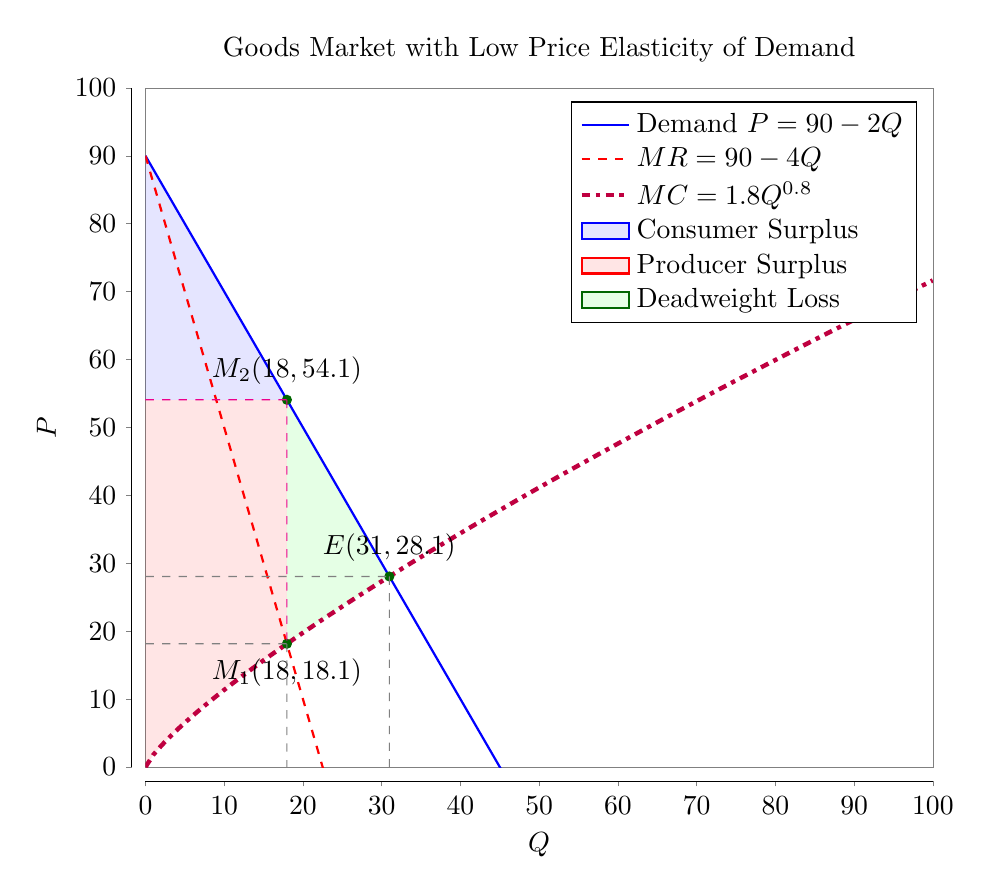
\begin{tikzpicture}

\begin{axis}[
    xmin = 0,
    xmax = 100,
    ymin = 0,
    ymax = 100,
    xlabel = {$Q$},
    ylabel = {$P$},
    sciclean/.style={axis lines=left,
        axis x line shift=0.5em,
        axis y line shift=0.5em,
        axis line style={-,very thin},
        axis background/.style={draw,ultra thin,gray},
        tick align=outside,
        major tick length=2pt},
    xtick distance=10,
    ytick distance=10,
    title = {Goods Market with Low Price Elasticity of Demand},
    domain = 0:100,
    legend cell align = left,
    % legend pos = south east,
    sciclean]

    \addplot[name path = D, thick, color = blue, samples = 100] {90 - 2*x};
    \addlegendentry{Demand $P = 90 - 2Q $}

    \addplot[name path = MR, dashed, thick, color = red, samples = 100] {90 - 4*x};
    \addlegendentry{$MR = 90 -4Q $}

    \addplot[name path = MC, ultra thick, color = purple, dashdotted, samples = 100] {1.8*x^0.8};
    \addlegendentry{$ MC = 1.8 Q^{0.8} $}

    \path[name intersections={of = MC and D, by=DMC}];
    \Getxycoords{DMC}{\xDRC}{\yDRC}
    \node[fill=black!60!green,circle,inner sep=1.3pt, label={[align=left]
        90:$E (\pgfmathprintnumber[precision=1]{\xDRC}, \pgfmathprintnumber[precision=1]{\yDRC})$ }] at (DMC)  {};
    \draw[name path = Line, dashed, gray] (0, \yDRC) -- (DMC);
    \draw[dashed, gray] (DMC) -- (\xDRC, 0);

    \path[name intersections={of = MC and MR, by=MRMC}];
    \Getxycoords{MRMC}{\xRC}{\yRC}
    \node[fill=black!60!green,circle,inner sep=1.3pt, label={[align=left]
        270:$M_{1} (\pgfmathprintnumber[precision=1]{\xRC}, \pgfmathprintnumber[precision=1]{\yRC})$ }] at (MRMC)  {};
    \draw[name path = Line2, dashed, gray] (0, \yRC) -- (MRMC);
    \draw[dashed, gray] (MRMC) -- (\xRC, 0);

    \path[name path = xM] (\xRC, 0) -- (\xRC, 100);
    \path[name intersections={of = D and xM, by=DxM}];
    \Getxycoords{DxM}{\xRC}{\yRC}
    \node[fill=black!60!green,circle,inner sep=1.3pt, label={[align=left]
        90:$M_{2} (\pgfmathprintnumber[precision=1]{\xRC}, \pgfmathprintnumber[precision=1]{\yRC})$ }] at (DxM)  {};
    \draw[name path = Line3, dashed, magenta] (0, \yRC) -- (DxM);
    \draw[name path = Line4, dashed, magenta] (DxM) -- (MRMC);

    \path[name intersections={of = Line4 and Line , by=Mid}];
    \Getxycoords{Mid}{\xRC}{\yRC}
    % \node[fill=black!60!green,circle,inner sep=1.3pt, label={[align=left]
    %     60:$M_{3}$ }] at (Mid)  {};

    \addplot [ thick, color=blue, fill=blue, fill opacity=0.1 ]
        fill between[
            of=D and Line3,
            soft clip={domain=0:100},
        ];
    \addlegendentry{Consumer Surplus}

    \addplot [ thick, color=red, fill=red, fill opacity=0.1 ]
        fill between[
            of=MC and Line3,
            soft clip={domain=0:\xRC},
        ];
    \addlegendentry{Producer Surplus}

    \addplot [ thick, color=black!60!green, fill=green, fill opacity=0.1 ]
        fill between[
            of=MC and D,
            soft clip={domain=\xRC:\xDRC},
        ];
    \addlegendentry{Deadweight Loss}

    % \path [name path = path10] (10,0) -- (10,100);

    % \path[name intersections={of = path10 and D, by=DMC}];
    % \node[fill=black!60!green,circle,inner sep=1.3pt, label={[align=left] 90:$A$ }] at (DMC)  {};

    % \path[name intersections={of = path10 and MC, by=SMC}];
    % \node[fill=black!60!green,circle,inner sep=1.3pt, label={[align=left] 270:$A'$ }] at (SMC)  {};
    % \draw[dashed, black!60!green] (DMC) -- (SMC);

    % \path [name path = path20] (20,0) -- (20,100);

    % \path[name intersections={of = path20 and D, by=DMC}];
    % \node[fill=black!60!green,circle,inner sep=1.3pt, label={[align=left] 90:$B$ }] at (DMC)  {};
    % \path[name intersections={of = path20 and MC, by=SMC}];
    % \node[fill=black!60!green,circle,inner sep=1.3pt, label={[align=left] 270:$B'$ }] at (SMC)  {};
    % \draw[dashed, black!60!green] (DMC) -- (SMC);

    % \path [name path = path30] (30,0) -- (30,100);
    % \path[name intersections={of = path30 and D, by=DMC}];
    % \node[fill=black!60!green,circle,inner sep=1.3pt, label={[align=left] 90:$C$ }] at (DMC)  {};
    % \path[name intersections={of = path30 and MC, by=SMC}];
    % \node[fill=black!60!green,circle,inner sep=1.3pt, label={[align=left] 270:$C'$ }] at (SMC)  {};
    % \draw[dashed, black!60!green] (DMC) -- (SMC);

    % \path [name path = path40] (40,0) -- (40,100);
    % \path[name intersections={of = path40 and D, by=DMC}];
    % \node[fill=black!60!green,circle,inner sep=1.3pt, label={[align=left] 90:$D$ }] at (DMC)  {};
    % \path[name intersections={of = path40 and MC, by=SMC}];
    % \node[fill=black!60!green,circle,inner sep=1.3pt, label={[align=left] 270:$D'$ }] at (SMC)  {};
    % \draw[dashed, black!60!green] (DMC) -- (SMC);

\end{axis}


\end{tikzpicture}

\end{document}

